In the past few weeks, we learned how to integrate functions $f : \R^n \to \R$ on curves, surfaces, and manifolds.
    
    \vspace{.5em}
    
    Now, we will learn how to integrate functions of the form $F: \R^n \to \R^n$ (also known as \textbf{vector fields}).  The resulting integrals are called \textbf{flow} and \textbf{flux} integrals.

\section{Vector fields}

\begin{definition}
    A vector field in $\R^n$ is a function $\bm{F} : \R^n \to \R^n$.  $\bm{F}$ assigns a vector $\bm{F}(\bm{P}) \in \R^n$ to every point $\bm{P}\in \R^n$.

\end{definition}

\begin{example}

    If $n=2$, then $$\bm{F}(x,y) = \langle F_1(x,y), F_2(x,y)\rangle$$
    
    If $n=3$, then $$\bm{F}(x,y,z) = \langle F_1(x,y,z), F_2(x,y,z), F_3(x,y,z)\rangle$$
    
\end{example}

\begin{example}[Constant vector field]
    
    Consider the vector field $\bm{F}(x,y) = \langle \frac{1}{2}, \frac{1}{2}\rangle$

    \begin{center}
        \begin{tikzpicture}[scale=0.75]
\begin{axis}[view={0}{90},domain=-2:2]
\addplot3 [UCLAblue,-latex,samples=8,
        quiver={
            u={1/2},
            v={1/2},
        },
    ] { 1}; % use pow(x^2 + y^2,1/2) if you choose to have a real 3D plot
\end{axis}
\end{tikzpicture}
    \end{center}

\end{example}

\begin{example}
    $$\bm{F} = \bm{i} + x\bm{j}$$

\begin{center}
    \begin{tikzpicture}
\begin{axis}[view={0}{90},domain=-4:4]
\addplot3 [UCLAblue,-latex,samples=10,
        quiver={
            u={1},
            v={x},
            scale arrows=0.3,
        },
    ] { 1};
\end{axis}
\end{tikzpicture}
    \end{center}
    
\end{example}

\begin{example}
    $$\bm{G} = \langle -y, x \rangle$$

\begin{center}
    \begin{tikzpicture}
\begin{axis}[view={0}{90},domain=-4:4]
\addplot3 [UCLAblue,-latex,samples=10,
        quiver={
            u={-y},
            v={x},
            scale arrows=0.3,
        },
    ] { 1};
\end{axis}
\end{tikzpicture}
    \end{center}
    
\end{example}

\begin{definition}
        A \textbf{unit vector field} is a vector field $\bm{F}$ such that $||\bm{F}(\bm{P})|| = 1$ for all $\bm{P} \in \R^n$.
    \end{definition}

\begin{definition}
    A \textbf{radial vector field} is a vector field $\bm{F}$ if for all $\bm{P}\in \R^n$, 
    \begin{enumerate}
        \item $\bm{F}(\bm{P})$ is parallel to the position vector $\bm{OP}$, AND
        \item $||\bm{F}(\bm{P})||$ depends only on $||\bm{OP}||$.
    \end{enumerate}
\end{definition}

\begin{example}
    \begin{center}
        \begin{tikzpicture}
\begin{axis}[view={0}{90},domain=-4:4]
\addplot3 [UCLAblue,-latex,samples=16,
        quiver={
            u={2*x/pow(x^2 + y^2,1/2)},
            v={2*y/pow(x^2 + y^2,1/2)},
            scale arrows=0.2,
        },
    ] { 1}; % use pow(x^2 + y^2,1/2) if you choose to have a real 3D plot
\end{axis}
\end{tikzpicture}
    \end{center}
\end{example}

\begin{example}
    \begin{center}
        \begin{tikzpicture}
  \begin{axis}[
    domain=-1:1,
    samples=10,
    xmin=-1,xmax=1,
    ymin=-1,ymax=1,
    zmin=-1,zmax=1,
    ]
    \pgfplotsinvokeforeach{-1,-.5,0,.5,1}{
      \addplot3[UCLAblue,-latex,
      point meta={sqrt((x)^2+(y)^2+(z)^2)},
      quiver={
        u={x/sqrt((x)^2+(y)^2+(z)^2)},
        v={y/sqrt((x)^2+(y)^2+(z)^2)},
        w={z/sqrt((x)^2+(y)^2+(z)^2)},
        scale arrows=.2}]
      (x,y,#1);
    }
  \end{axis}
\end{tikzpicture}
    \end{center}
\end{example}

\subsection{Operations on vector fields}

An important class of examples of vector fields in $\R^n$ are conservative vector fields, which come from smooth (though we technically only need $C^1$) functions $f: \R^n \to \R$.  Recall that the gradient of a multivariable function is denoted $\nabla$ (and is also sometimes called the del operator)

\begin{definition}
    Let $f: \R^n \to \R$ be a differentiable function.  Consider the gradient operator $\nabla$ defined by
    $$\nabla f (\bm{u}) = \langle \frac{\partial f}{\partial x_1}(\bm{u}), \cdots , \frac{\partial f}{\partial x_n}(\bm{u}) \rangle$$
    
    Observe that $\nabla$ turns a scalar function $f: \R^n \to \R$ into a vector field $F: \R^n \to \R^n$.
    \end{definition}

\begin{definition}
    A vector field $\bm{F} : \R^n \to \R^n$ is called \textbf{conservative} if there is a differentiable function $f(x_1,\cdots, x_n)$ such that $$\bm{F} = \nabla f = \langle \frac{\partial f}{\partial x_1}, \cdots , \frac{\partial f}{\partial x_n} \rangle$$
    $f$ is called a \textbf{potential function} for $\bm{F}$.
    \end{definition}








\begin{definition}
    Given a vector field $\bm{F} : \R^n \to \R^n$ defined by $$\bm{F}(\bm{u}) = \langle F_1(\bm{u}),\cdots, F_n(\bm{u}) \rangle$$ the \textbf{divergence of} $\bm{F}$ is the scalar-valued function $f : \R^n \to \R$ defined by     
    $$\textnormal{div} \bm{F}(\bm{u}) = \frac{\partial F_1}{\partial x_1}(\bm{u}) + \cdots + \frac{\partial F_n}{\partial x_n}(\bm{u})$$
    \end{definition}

Observe that we can abuse notation by writing $$\textnormal{div} \bm{F} = \nabla \cdot \bm{F} = \langle\frac{\partial}{\partial x}, \frac{\partial}{\partial y}, \frac{\partial}{\partial z}  \rangle \cdot \bm{F} $$
    
    Of course, $\nabla = \langle\frac{\partial}{\partial x}, \frac{\partial}{\partial y}, \frac{\partial}{\partial z}  \rangle$ is an operator, \underline{not} a vector, and so it doesn't literally make sense to take the dot product with $\nabla$. 


\begin{example}
    Calculate the divergence of $\bm{F} = \langle e^{xy}, xy, z^4 \rangle$ at the point $P = (1,0,2)$.
\end{example}






\begin{remark}
    The divergence of a vector field at a point $P$ measures the flux of $\bm{F}$ through a sphere of radius $\varepsilon$ around $P$. 
    
    \begin{enumerate}
        \item If $\textnormal{div} \bm{F} > 0$, then $P$ is a source.
        \item If $\textnormal{div} \bm{F} < 0$, then $P$ is a sink.
        \item If $\textnormal{div} \bm{F} = 0$, then $P$ is said to be incompressible.
    \end{enumerate}
    \end{remark}
    
%\begin{center}
%        % RADIAL OUTWARD
%\begin{tikzpicture}
%  \fill[red] (0,0) circle (\r);
%  \foreach \i [evaluate={\ang=\i*360/\N;}] in {0,...,\N}{
%    \draw[vector] (\ang:0.1*\D) --++ (\ang:\D);
%  }
%  \node at (0,-1.35*\D) {$\textnormal{div} \bm{F} > 0$};
%\end{tikzpicture}
%% RADIAL INWARD
%\begin{tikzpicture}
%  \fill[red] (0,0) circle (\r);
%  \foreach \i [evaluate={\ang=\i*360/\N;}] in {0,...,\N}{
%    \draw[vector] (\ang:1.1*\D) -- (\ang:0.1*\D);
%  }
%  \node at (0,-1.35*\D) {$\textnormal{div} \bm{F} < 0$};
%\end{tikzpicture}
%% ZERO
%\begin{tikzpicture}
%  \def\ang{60}
%  \fill[red] (0,0) circle (\r);
%  \foreach \x/\y in {-1/0,-1/1,0/1,1/1,1/0,-1/-1,0/-1,1/-1}{
%    \draw[vector] (\x*0.5*\D,\y*0.5*\D) ++ (\ang-180:\D/2) --++ (\ang:\D);
%  }
%  \node at (0,-1.35*\D) {$\textnormal{div} \bm{F} = 0$};
%\end{tikzpicture}
%\end{center}


\begin{definition}
    Given a vector field in $\R^3$, $\bm{F} = \langle F_1, F_2, F_3 \rangle$, the \textbf{curl of} $\bm{F}$ is the vector field defined by 
    
    $$\textnormal{curl} \bm{F} = \langle \frac{\partial F_3}{\partial y} - \frac{\partial F_2}{\partial z}, \frac{\partial F_1}{\partial z} - \frac{\partial F_3}{\partial x}, \frac{\partial F_2}{\partial x} - \frac{\partial F_1}{\partial y} \rangle $$
    \end{definition}

Observe that we can abuse notation by writing $$\textnormal{curl} \bm{F} = \nabla \times \bm{F} = \langle\frac{\partial}{\partial x}, \frac{\partial}{\partial y}, \frac{\partial}{\partial z}  \rangle \times \bm{F} $$
    
    Of course, this also doesn't make literal sense. 

\begin{example}
    Calculate the curl of $\bm{F} = \langle xy, e^x,y+z \rangle$  at the point $P = (1,0,2)$.
\end{example}





\begin{example}
    
    Consider the vector field $\bm{F}(x,y,z) = \langle -y, x, 0 \rangle$ pictured on the left, with curl $\bm{F}$ on the right)
    
    \begin{center}
    \begin{tikzpicture}[scale=0.75]
  \begin{axis}[
    domain=-1:1,
    samples=7,
    xmin=-1,xmax=1,
    ymin=-1,ymax=1,
    zmin=-1,zmax=1,
    ]
    \pgfplotsinvokeforeach{-1,-.5,0,.5,1}{
      \addplot3[UCLAblue,quiver,-stealth,
      quiver={
        u={-y},
        v={x},
        w={0},
        scale arrows=.2}]
      (x,y,#1);
    }
  \end{axis}
\end{tikzpicture}
\begin{tikzpicture}[scale=0.75]
  \begin{axis}[
    domain=-1:1,
    samples=5,
    xmin=-1,xmax=1,
    ymin=-1,ymax=1,
    zmin=-1,zmax=1,
    ]
    \pgfplotsinvokeforeach{-1,-.5,0,.5,1}{
      \addplot3[UCLAblue,quiver,-stealth,
      quiver={
        u={0},
        v={0},
        w={2},
        scale arrows=.2}]
      (x,y,#1);
    }
  \end{axis}
\end{tikzpicture}
    \end{center}
    \end{example}

The geometric interpretation of the curl is as follows:  Imagine a ball is fixed at a point $P$ in a vector field $\bm{F}$.  Then if the vector field causes the ball to rotate, then the vector $\textnormal{curl}\bm{F}(P)$ points in the direction of the axis of counterclockwise rotation.   
    Moreover, the angular speed of rotation is directly proportional to the magnitude of $\textnormal{curl}\bm{F}(P)$.







\subsection{Exercises}


\section{Vector line integrals}


\begin{motivating}
    How can we set up for the fundamental theorem of calculus?
\end{motivating}


\begin{remark}
        Observe that in single variable calculus, there is a relationship between
        $$\int_a^b f(x) \ dx \qquad \textnormal{and} \qquad \int_b^a f(x) \ dx$$

From our setup of integration, the latter is meaningless - the set $\{x \in \R \ | \ b  \leq x \leq a\}$ is the empty set.
    
    \vspace{.5em}
    
    However, we have an intuitive idea of what $[b,a]$ should mean - it should mean going from $b$ to $a$, or equivalently, travelling along $[a,b]$ in the negative (or opposite) direction.  To make this precise, we need the idea of \textbf{orientations}.

        \end{remark}

In $\R$, there is a natural choice of orientation by choosing the positive real numbers to be the positive direction, and the negative numbers to be the negative direction.

\begin{definition}
    Given a curve $C$, a continuous choice of tangent vector on $C$ is called an \textbf{orientation}.
    
    \vspace{.5em}
    
    A curve with a chosen orientation is called an \textbf{oriented curve}.
    
    
    
    \vspace{.5em}
    
    Going along the choice of direction is called the \textbf{positive direction along} $C$, and going against the choice of orientation is called the \textbf{negative direction} (along $C$).
    \end{definition}







\subsection{Vector flow line integrals}


\begin{motivating}
    How do we integrate vector fields over curves?
\end{motivating}

\begin{definition}
    Given an oriented curve $C$, let $\bm{T}(p)$ denote the unit tangent vector of $C$ at the point $p$, pointing in the positive direction.  
    
    \vspace{.5em}
    
    Let $\bm{F}$ be a vector field.  The \textbf{tangential component} of $\bm{F}$ at $p$ is the dot product 
    $$\bm{T}(p) \cdot \bm{F}(p)$$
    
    \end{definition}

\begin{definition}
        The \textbf{line integral of a vector field} $\bm{F}$ along an oriented curve $C$ is denoted $\int_C \bm{F} \cdot d\bm{r}$.  We define it as the integral of the tangential component of $\bm{F}$ over $C$.
        
    $$\int_C \bm{F} \cdot d\bm{r} := \int_C (\bm{F} \cdot \bm{T}) \ ds $$
    \end{definition}

\begin{example}
    The work $W$ performed \textbf{by} a vector field $F$ on an object moving along a curve $C$ is given by $$W = \int_C \bm{F} \cdot d\bm{r}$$
    \end{example}



    \begin{example}
    The work $W$ performed \textbf{against} a vector field $F$ by moving an object along a curve $C$ is given by $$W = - \int_C \bm{F} \cdot d\bm{r}$$
    \end{example}

\begin{theorem}
    Let $\bm{r}(t)$ be a positively oriented regular parametrization of an oriented curve $C$ for $a \leq t \leq b$.  Then
    $$\int_C \bm{F} \cdot d\bm{r} = \int_a^b \bm{F}(\bm{r}(t)) \cdot \bm{r}'(t) \ dt$$
    
    \end{theorem}
    
\begin{proof}
\end{proof}

    
    \begin{remark} If $\bm{F} = \langle F_1, F_2, F_3 \rangle$, then another common notation for line integrals is 
    $$\int_C \bm{F} \cdot d\bm{r} = \int_C F_1 \ dx + F_2 \ dy + F_3 \ dz$$
    
    \end{remark}

\begin{example}
    Consider the vortex field $\bm{F} = \langle \frac{-y}{x^2 + y^2}, \frac{x}{x^2 + y^2} \rangle$. Compute $$\int_C \bm{F} \cdot d\bm{r}$$ for $C$ is the circle of radius $R$ centered at the origin, oriented counterclockwise.


\begin{center}
        \begin{tikzpicture}
\begin{axis}[view={0}{90},domain=-4:4]
\addplot3 [UCLAblue,-latex,samples=16,
        quiver={
            u={-2*y/(x^2 + y^2)},
            v={2*x/(x^2 + y^2)},
            scale arrows=0.5,
        },
    ] { 1}; % use pow(x^2 + y^2,1/2) if you choose to have a real 3D plot
\end{axis}
\end{tikzpicture}
    \end{center}
\end{example}


\begin{theorem}[Properties of Vector Line Integrals]
    Let $C$ be a smooth oriented curve, and let $\bm{F}$ and $\bm{G}$ be vector fields.
    
    \begin{enumerate}
        \item \textbf{Linearity:} $$\int_C \bm{F+G} \cdot d\bm{r} = \int_C \bm{F} \cdot d\bm{r} + \int_C \bm{G} \cdot d\bm{r}$$

        $$\lambda \int_C \bm{F} \cdot d\bm{r} = \int_C \lambda\bm{F} \cdot d\bm{r} $$
        \item \textbf{Additivity}:  If $C$ is the union of smooth curves $C_1 \cup \cdots \cup C_n$, then 
        $$\int_C \bm{F} \cdot d\bm{r} = \int_{C_1} \bm{F} \cdot d\bm{r} + \cdots + \int_{C_n} \bm{F} \cdot d\bm{r}$$
        
        \item \textbf{Reversing orientation}:  $$\int_{-C} \bm{F} \cdot d\bm{r} =  -\int_C \bm{F} \cdot d\bm{r}$$
        
    \end{enumerate}
    
    \end{theorem}


\subsubsection{Integrating Conservative Vector Fields}

\begin{definition}
    A vector field $\bm{F} : D \subset \R^n \to \R^n$ is called \textbf{conservative} if there is a differentiable function $f(x_1,\cdots, x_n) : D \to \R$ such that $$\bm{F} = \nabla f = \langle \frac{\partial f}{\partial x_1}, \cdots , \frac{\partial f}{\partial x_n} \rangle$$
    $f$ is called a \textbf{(scalar) potential function} for $\bm{F}$.
    \end{definition}
    
    \begin{theorem}[Uniqueness of potential functions]\label{uniquenesspotential}
    If $\bm{F}$ is a conservative vector field on an open, connected domain $U$, then any two potential functions of $\bm{F}$ differ by a constant.
    \end{theorem}

    You will see in lecture how this can help us integrate conservative vector fields over curves! You should think of this theorem as a generalization of the following theorem from single variable calculus: 

    \begin{theorem}
    If $f: \R \to \R$ is a function on an open interval $(a,b)$, then any two antiderivatives of $f$ differ by a constant.
    \end{theorem}

\begin{theorem}[Fundamental Theorem for Conservative Vector Fields]
    Let $\bm{F} = \nabla f$ be a conservative vector field on a domain $D$. If $\bm{r}$ is a path along a curve $C$ from $P$ to $Q$ in $D$, then $$\int_C \bm{F} \cdot d\bm{r} = f(Q) - f(P)$$
    In particular, $\bm{F}$ is path-independent.
    \end{theorem}


\begin{example}
    Let $\bm{F}(x,y,z) = \langle 2xy + z, x^2, x \rangle$.  Compute $$\int_C \bm{F} \cdot d\bm{r}$$ for $C$ the straight line from $(1,-1,2)$ to $(2,2,3)$
\end{example}

\begin{corollary}
    Let $\bm{F} = \nabla f$ be a conservative vector field on a domain $D$. If $\bm{r}$ is a path along a \textbf{closed curve} $C$ in $D$, then the circulation is zero:
    $$\oint_C \bm{F} \cdot d\bm{r} = 0$$
    \end{corollary}

\begin{example}
    Let $\bm{F}(x,y,z) = \langle y\sin(yz), xyz\cos(yz) + x\sin(yz), xy^2\cos(yz) \rangle$.  Compute $$\oint_C \bm{F} \cdot d\bm{r}$$ for $C$ the curve below:
    
%    \begin{figure}
%        \centering
%        \includegraphics[scale=0.3]{pictures/conservativecurve.png}
%    \end{figure}
\end{example}

\begin{motivating}
    How can we identify conservative vector fields?
\end{motivating}

\begin{theorem}
    If $\bm{F} = \nabla f$ is a conservative vector field, then $\textnormal{curl} (\nabla f) = \bm{0}$.
\end{theorem}



\begin{theorem}
    Let $\bm{F}$ be a vector field on a \textbf{simply-connected} domain $D$. If $\bm{F}$ satisfies the cross-partials condition, then $\bm{F}$ is conservative.
    \end{theorem}

\begin{example}
     The vortex field $\bm{F} = \langle \frac{-y}{x^2 + y^2}, \frac{x}{x^2 + y^2} \rangle$, defined on $\R^2 - \{(0,0)\}$, satisfies the cross partials condition, but is not conservative on $\R^2 - \{(0,0)\}$.

     \begin{center}
        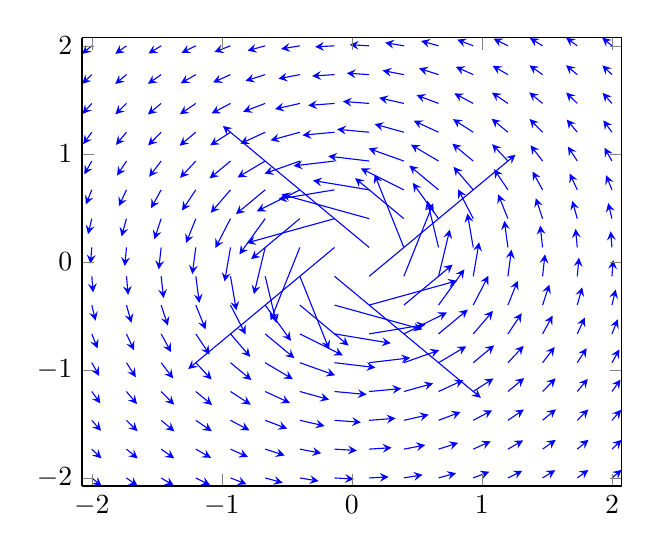
\begin{tikzpicture}
\begin{axis}[view={0}{90},domain=-2:2]
\addplot3 [blue,-stealth,samples=16,
        quiver={
            u={-1*y/(x^2 + y^2)},
            v={x/(x^2 + y^2)},
            scale arrows=0.3,
        },
    ] { 1}; % use pow(x^2 + y^2,1/2) if you choose to have a real 3D plot
\end{axis}
\end{tikzpicture}
    \end{center}
\end{example}

\begin{example}
    However, the vortex field $\bm{F} = \langle \frac{-y}{x^2 + y^2}, \frac{x}{x^2 + y^2} \rangle$ \textbf{is conservative} on $\{(x,y) \ | \ x > 0\}$.
\end{example}


\begin{definition}
    A vector field $\bm{F}$ on a domain $D$ is \textbf{path-independent} if for any two points $\bm{P}, \bm{Q} \in D$, then 
    $$\int_{C_1} \bm{F} \cdot d\bm{r} = \int_{C_2} \bm{F} \cdot d\bm{r}$$
    For any two paths $C_1, C_2$ in $D$ that start at $\bm{P}$ and end at $\bm{Q}$.
\end{definition}
    
    \begin{motivating}
        Are there any non-conservative path-independent vector fields?
    \end{motivating}
    
       
    \begin{theorem}
    A vector field $\bm{F}$ in an open, connected domain $D$ is path-independent if and only if it is conservative.
    \end{theorem}

    \begin{proof}
        
    \end{proof}


\subsection{Vector flux line integrals}

\begin{motivating}
    Imagine that $C$ is a cell membrane - how much water flows through $C$?
\end{motivating}

\begin{motivating}
    How do we compute flux line integrals?
\end{motivating}

\begin{definition}
    Given an oriented curve $C$ in $\R^2$, we say that the \textbf{positive direction \textit{across} $C$} is the direction that goes left to right from the perspective of the positive orientation \textit{along $C$}.
        
    %\pause
    
    
    Let $\bm{n}(p)$ denote the unit vector normal to $C$ at the point $p$, pointing in the positive direction across $C$.  
    
    \end{definition}

\begin{definition}
    Let $\bm{F}$ be a vector field.  The \textbf{normal component} of $\bm{F}$ at $p \in C$ is the dot product 
    $$\bm{n}(p) \cdot \bm{F}(p)$$
    
    \end{definition}

\begin{theorem}
    The \textbf{flux integral} of a vector field $\bm{F}$ along an oriented curve $C$ in $\R^2$ is the integral of the normal component of $\bm{F}$:
    $$\int_C \bm{F} \cdot \bm{n} \ ds$$
    
    \end{theorem}

\begin{remark}
    Let $\bm{r}(t) = \langle x(t), y(t)\rangle$ be a positive oriented regular parametrization of an oriented curve $C$. Observe that $\bm{N}(t) = \langle y'(t), -x'(t) \rangle$ is normal to $C$.  Therefore,
    $$\bm{n}(t) = \frac{\bm{N}(t)}{||\bm{N}(t)||}$$
    \end{remark}

\begin{theorem}
    Let $\bm{r}(t) = \langle x(t), y(t)\rangle$ be a positive oriented regular parametrization of an oriented curve $C$ for $a \leq t \leq b$.  Then
    $$\int_C \bm{F} \cdot \bm{n} \ ds = \int_a^b \bm{F}(\bm{r}(t)) \cdot \bm{N}(t) \ dt$$
    
    \end{theorem}

\begin{example}
    Calculate the flux of the velocity vector field $\bm{v} = \langle 3+2y -\frac{y^2}{3}, 0 \rangle$ (in cm/sec) across the quarter ellipse $\bm{r}(t) = \langle 3\cos(t), 6\sin(t) \rangle$ for $0 \leq t \leq \frac{\pi}{2}$.
\end{example}



\subsection{Exercises}

\begin{problem}
    Let $\bm{F}(x,y) = \langle \frac{1}{x}, \frac{-1}{y} \rangle$.  Calculate the work against $F$ required to move an object in from $(1,1)$ to $(2,4)$ along the parabola $y=x^2$, and from $(2,4)$ to $(3,4)$ along a straight line path.
\end{problem}

\begin{problem}
    Consider the unit cube of vertices at the points $(0,0,0)$ and $(1,1,1)$.  Pick any path along the edges of the cube that starts at $(0,0,0)$ and ends at $(1,1,1)$.  Let $\bm{F}(x,y,z) = \langle e^z, e^{x-y}, e^y \rangle$.  Calculate the line integral of $\bm{F}$ along your chosen path.
\end{problem}

\begin{problem}
    Consider the triangle with vertices $A = (2,0,0)$, $B = (0,4,0)$, $C = (0,0,6)$.  Let $\bm{F}(x,y,z) = \langle e^z, e^{x-y}, e^y \rangle$.  Calculate the line integral of $\bm{F}$ along the closed loop $ABCA$.
\end{problem}

\begin{problem}{conservative1}
Let $\bm{F} = \langle 2x+y, x \rangle$, and calculate $\int_C \bm{F} \cdot d\bm{r}$, where $\bm{r}$ is any path from $(1,2)$ to $(5,7)$.
\end{problem}

\begin{problem}{vortexconservative}
    Consider the vortex field $\bm{F} = \langle \frac{-y}{x^2 + y^2}, \frac{x}{x^2 + y^2} \rangle$ on the region $\{(x,y) \ | \ x > 0\}$. Show that $\bm{F}$ is conservative on this region.  (\textbf{Hint:} Consider the function $\tan^{-1}(u)$).
\end{problem}

\begin{problem}{flux1}
     Calculate the flux of the vector field $\bm{F} = \langle -y, x \rangle$ across the upper half of the unit circle centered at the origin, oriented clockwise.
\end{problem}

\begin{problem}{fluxparam2}
    Find a positively oriented parametrization of the parabola $y = x^2$ for $0 \leq x \leq 1$, oriented from left to right (from $(0,0)$ to $(1,1)$). 
\end{problem}

\begin{problem}{flux2}
    Compute the flux of the vector field $\bm{F} = \langle e^y, 2x-1 \rangle$ across the parabola $y = x^2$ for $0 \leq x \leq 1$, oriented from left to right.
\end{problem}

\begin{problem}{fluxparam3}
    Find a positively oriented parametrization of the parabola $y = x^2$ for $0 \leq x \leq 1$, oriented from right to left (from $(1,1)$ to $(0,0)$). 
\end{problem}

\begin{problem}{flux3}
    Compute the flux of the vector field $\bm{F} = \langle e^y, 2x-1 \rangle$ across the parabola $y = x^2$ for $0 \leq x \leq 1$, oriented from right to left.
\end{problem}


\section{Vector surface integrals}

\begin{motivating}
    How do we compute surface integrals of vector fields?
\end{motivating}

\begin{definition}
    Let $S$ be a surface in $\R^3$. An orientation on $S$ is a continuous choice of a unit normal vector $\bm{n}(P)$ at each point $P$ on $S$.  We say that the \textbf{positive orientation \textit{across} $S$} is in the direction of the normal vector $\bm{n}$.
    
    We say that $-\bm{n}$ is the \textbf{opposite orientation} of $S$.
    
    
    We say that a surface with a choice of orientation is an \textbf{oriented surface}.
    
    \end{definition}

\begin{definition}
    Let $\bm{F}$ be a vector field in $\R^3$, and let $P = G(u_0,v_0)$ be a point on an oriented surface $S$.  The \textbf{normal component} of $\bm{F}$ at $p$ is the dot product 
    $$\bm{F}(P) \cdot \bm{n}(P)$$
    \end{definition}

\begin{definition}
    The \textbf{vector surface integral} of $\bm{F}$ over $S$ is defined as
    $$\iint_S \bm{F} \cdot d\bm{S} := \iint_S (\bm{F} \cdot \bm{n}) \ dS$$
    This is also known as the \textbf{flux} of $\bm{F}$ across (or through) $S$.
    \end{definition}

    \begin{definition}
    For a fluid with velocity vector field $\bm{v}$, the flow rate across $S$ (in volume/time) is given by 
    $$\iint_S \bm{v} \cdot d\bm{S}$$
    \end{definition}

\begin{theorem}
    If $-S$ denotes $S$ with the opposite orientation, then $$\iint_{-S} (\bm{F} \cdot \bm{n}) \ dS = -\iint_S (\bm{F} \cdot \bm{n}) \ dS$$
    \end{theorem}

Recall that given a \textbf{regular} parametrization $G(u,v)$ of $S$, then a normal vector at a point $P = G(u_0,v_0)$ on $S$ is determined by 
    $$\bm{N}(P) =  \frac{\partial G}{\partial u}(u_0,v_0) \times \frac{\partial G}{\partial v}(u_0,v_0)$$ 

\begin{definition}
    An \textbf{oriented parametrization} of a surface $S$ is a parametrization $G(u,v)$, with the orientation of $S$ determined by the unit normal vector $$\bm{n}(P) = \frac{\bm{N}(P)}{||\bm{N}(P)||}$$
    
    
    Given an oriented parametrization, we say that the \textbf{positive orientation \textit{of} $S$} is in the direction of the normal vector $\bm{N}$.
    
    \vspace{1em}
    
    $-\bm{N}$ gives the opposite (or negative) orientation of $S$.
    
    \end{definition}

\begin{remark}
    
    \textbf{Warning:} Not every surface is orientable, and not every parametrization is an oriented parametrization!    
    \end{remark}

\begin{center}
%    \begin{tikzpicture}[scale=0.6]
%    \begin{axis}[hide axis,
%    colormap/cool,view={60}{30}, width=15cm, axis equal image]
%        % Draw sphere (example from the pgfplots manual)
%        \addplot3[
%            surf, z buffer=sort, colormap/cool, point meta=-z,
%            samples=20, domain=-1:1, y domain=0:2*pi
%        ]
%        (
%            {(1+ x*cos(deg(y)/2))*cos(deg(y))}, % X coordinate
%            {(1+ x*cos(deg(y)/2))*sin(deg(y))}, % Y coordinate
%            sin(deg(y)/2)                           % Z (vertical) coordinate
%        );
%    \end{axis}
%\end{tikzpicture}
        
    \end{center}

 \begin{theorem}
    Let $G(u,v) : D \to \R^3$ be an oriented parametrization of a surface $S$.  Assume that $G$ is one-to-one and regular, except possibly at points on the boundary of $D$.  Then
    $$\iint_S (\bm{F} \cdot \bm{n}) \ dS = \iint_D \bm{F}(G(u,v)) \cdot \bm{N}(u,v) \ du \ dv$$
    
    \end{theorem}

\begin{example}
    Calculate $\iint_S \bm{F} \cdot d\bm{S}$, where $\bm{F} = \langle 0, 0, x\rangle$, and $S$ is the surface with parametrization $G(u,v) : D \to \R^3$, 
    $$G(u,v) = (u^2,v,u^3-v^2)$$
    for $D = \{(u,v) \ |\  0 \leq u \leq 1, \ 0 \leq v \leq 1\}$, and $S$ is oriented with upward-pointing normal vectors.
\end{example}

\subsection{Exercises}

\begin{problem}{surfaceflux1}
     Find a \textbf{positively oriented} parametrization of the upper hemisphere of the unit sphere, centered at the origin, with outward pointing normal vectors.
\end{problem}

\begin{problem}{surfaceflux2}
     Calculate the flux of $\bm{F} = \langle z, x, 1 \rangle$ across the upper hemisphere of the unit sphere, centered at the origin, with outward pointing normal vectors.
\end{problem}




\section{Green's theorem, Stokes' theorem, and the divergence theorem}

\begin{motivating}
    How can we generalize the fundamental theorem of single variable calculus?
\end{motivating}

\begin{theorem}[Fundamental Theorem for Conservative Vector Fields]
    Let $\bm{F} = \nabla f$ be a conservative vector field on a domain $D$. If $\bm{r}$ is a path along a \textbf{closed curve} $C$ in $D$, then the circulation is zero:
    $$\oint_C \bm{F} \cdot d\bm{r} = 0$$
    \end{theorem}

What if $\bm{F}$ is \textbf{not} conservative?  Can we still calculate $\oint_C \bm{F} \cdot d\bm{r}$?


\subsection{Green's theorem}


\begin{definition}
    A \textbf{simple} closed curve $C$ is a closed curve that does not intersect itself.
\end{definition}

\begin{theorem}[Green's theorem]
    Let $D$ be a region in $\R^2$ such that $\partial D$ is a disjoint union of simple closed curves, with $\partial D$ oriented so that $D$ is always to the left.
    
    \vspace{1em}
    
    
    Suppose $\bm{F} = \langle F_1, F_2 \rangle$ is a smooth vector field on $D$.  Then
    $$\oint_{\partial D} \bm{F} \cdot d\bm{r} = \iint_D \left(\frac{\partial F_2}{\partial x} - \frac{\partial F_1}{\partial y}\right) \ dA$$
    
    \end{theorem}


\begin{remark}
    Green's theorem is a generalization of the fundamental theorem for conservative vector fields.
\end{remark}

\begin{theorem}[Additivity of circulation]
    Let $D$ be a region in $\R^2$ such that $\partial D$ is a simple closed curve, oriented counterclockwise.  If we decomposes a domain $D$ into two domains $D_1$ and $D_2$ who intersect only on their boundaries, $\partial D_1$ and $\partial D_2$, then
    $$\oint_{\partial D} \bm{F} \cdot d\bm{r} = \oint_{\partial D_1} \bm{F} \cdot d\bm{r} + \oint_{\partial D_2} \bm{F} \cdot d\bm{r}$$
    
    \end{theorem}

%    \begin{figure}
%        \centering
%        \includegraphics[scale=0.4]{pictures/greenstheoremboundary.png}
%    \end{figure}
    
\begin{motivating}
How does Green's theorem relate to flux integrals and the divergence of a vector field in $\R^2$?
\end{motivating}


\begin{theorem}
    Let $\bm{r}(t) = \langle x(t), y(t)\rangle$ be a positive oriented regular parametrization of an oriented curve $C$ for $a \leq t \leq b$.  Then
    $$\int_C \bm{F} \cdot \bm{n} \ ds = \int_a^b \bm{F} \cdot \left\langle \frac{y'(t)}{||\bm{r}'(t)||}, \frac{-x'(t)}{||\bm{r}'(t)||} \right\rangle \ ||\bm{r}'(t)||\ dt$$
    Thus
    $$\oint_{\partial D} \bm{F} \cdot \bm{n} \ ds = \oint_{\partial D} F_1 \ dy - F_2 \ dx$$
    \end{theorem}

\begin{theorem}[Green's theorem, flux form]
    Let $D$ be a region in $\R^2$ such that $\partial D$ is a simple closed curve, oriented counterclockwise.  Suppose $\bm{F} = \langle F_1, F_2 \rangle$ is a smooth vector field on $D$.
    Then
    $$\oint_{\partial D} \bm{F} \cdot \bm{n} \ ds = \iint_D \textnormal{div}(\bm{F}) \ dA$$
        \end{theorem}

\begin{corollary}
    Suppose $\bm{F} = \langle F_1, F_2 \rangle$ is a smooth vector field, and let $P$ be a point in $\R^2$.  Let $D = B_\varepsilon(P)$ be a small disk around $P$. 
    
    Then
    $$\oint_{\partial D} \bm{F} \cdot \bm{n} \ ds = \iint_D \textnormal{div}(\bm{F}) \ dA \approx \textnormal{div}(\bm{F})(P) \cdot \textnormal{area}(D)$$

    Thus, $$\textnormal{div}(\bm{F})(P) \approx \frac{1}{\textnormal{area}(D)}\oint_{\partial D} \bm{F} \cdot \bm{n} \ ds$$
    Therefore, the divergence of a 2D vector field $\bm{F}$ measures the \textbf{outward flux} of $\bm{F}$.
    \end{corollary}

\begin{theorem}[Green's theorem, circulation form]
    Let $D$ be a region in $\R^2$ such that $\partial D$ is a simple closed curve, oriented counterclockwise.  Suppose $\bm{F} = \langle F_1, F_2 \rangle$ is a smooth vector field on $D$.
    Then
    $$\oint_{\partial D} \bm{F} \cdot d\bm{r} = \iint_D \textnormal{curl}_z(\bm{F}) \ dA$$
        \end{theorem}

\begin{corollary}
    Suppose $\bm{F} = \langle F_1, F_2 \rangle$ is a smooth vector field, and let $P$ be a point in $\R^2$.  Let $D = B_\varepsilon(P)$ be a small disk around $P$. 
    
    Then
    $$\oint_{\partial D} \bm{F} \cdot d\bm{r} = \iint_D \textnormal{curl}_z(\bm{F}) \ dA \approx \textnormal{curl}_z(\bm{F})(P) \cdot \textnormal{area}(D)$$

    Thus, $$\textnormal{curl}_z(\bm{F})(P) \approx \frac{1}{\textnormal{area}(D)}\oint_{\partial D} \bm{F} \cdot d\bm{r}$$
    Therefore, the curl of a 2D vector field $\bm{F}$ measures the \textbf{circulation} of $\bm{F}$.
    \end{corollary}

\subsection{Stokes' theorem}

\begin{motivating}
    Is there an analogue or generalization of Green's theorem in 3 dimensions?
\end{motivating}

\begin{remark}
    A \textbf{simple} closed curve $C$ in $\R^3$ can be thought of as the boundary of a surface $S$ in $\R^3$.
    \end{remark}

\begin{definition}
    A subset $M \subset \R^n$ is a \textbf{differentiable $k$-dimensional manifold \textit{with boundary}} embedded in $\R^n$  if for all $\bm{z} \in M$, \underline{either}
    
    \begin{enumerate}
        \item  there exists an open neighborhood $U \subset \R^n$ such that there exists a $C^1$-mapping $F : U \to \R^{n-k}$ such that
                \begin{itemize}
            \item $M \cap U = \{\bm{z} \in U \ | \ F(\bm{z}) = \bm{0} \}$
            \item $[DF(\bm{z})]$ is surjective
        \end{itemize}

        \item \underline{OR} there exists an open neighborhood $V \subset \R^n$ such that there exists a $C^1$-mapping $G : V \to \R^{m}$ such that
        \begin{itemize}
            \item $G(\bm{z}) = \bm{0}$
            \item $M \cap V = \{\bm{x} \in V \ | \ G(\bm{x}) \geq \bm{0} \}$
            \item $[DG(\bm{z})]$ is surjective
        \end{itemize}
    \end{enumerate}

    We say that the set of points $\bm{z} \in M$ satisfying the latter condition are the boundary of $M$.  
    \end{definition}

\begin{example}
    The \textbf{upper half-space} $H^k \subset \R^k$ is the (closed) set $$H^k := \{ \bm{x} = \langle x_1, \cdots, x_k \rangle \ | \ x_k \geq 0\}$$
    This is a $k$-dimensional manifold with boundary $$\partial H^k =\{ \langle x_1, \cdots, x_k \rangle \ | \ x_k = 0\} $$
    \end{example}

\begin{example}
     What is the boundary of the hemisphere? $$S_+ = \{(x,y,z) \ | \ x^2 + y^2 + z^2 = 1, z \geq 0\}$$
\end{example}

\begin{example}
    
    What is the boundary of the solid cube in $\R^3$?
\end{example}

\begin{definition}
        If $\bm{z} \in \partial M$ satisfies the latter condition, we say that $\bm{z}$ is a \textbf{corner point of codimension $m$}.
        
        \vspace{1em}
        
        In the special case $m = 1$, then we say that $\bm{z}$ is in the \textbf{smooth boundary} of $M$ (denoted $\partial^s M$).
        
        \vspace{1em}
        
        The set of corner points that is not in $\partial^s M$ is called the \textbf{non-smooth boundary} of $M$.
    \end{definition}

\begin{proposition}
    The smooth boundary $\partial^s M$ is a $k-1$-dimensional manifold.
    \end{proposition}


    \begin{proposition}
    The non-smooth boundary of $M$ has $(k-1)$-dimensional volume 0.
    \end{proposition}

Recall that an orientation of a surface $S$ in $\R^3$ is a (continuous) choice of a unit normal vector $\bm{n}(P)$ at each point $P$ on $S$.  If $S$ is an oriented surface, then we can specify an orientation of the boundary $\partial S$.

\begin{definition}
    
    The \textbf{boundary orientation} of $\partial S$ is chosen so that if your feet are $S$, and your head is where the head of $\bm{n}(P)$ is, then the orientation of $\partial S$ is chosen so that $S$ is always to your left.
    
\end{definition}

\begin{theorem}[Stoke's Theorem]
    Let $G(u,v) : D \to \R^3$ be a positively oriented parametrization of a surface $S$.  Assume that $G$ is one-to-one and regular, except possibly at points on the boundary of $D$.  This determines an orientation on $\partial S$.
    
    \vspace{1em}
    
    Suppose $\bm{F}$ is a smooth vector field on a solid region $W$ containing $S$. Then
    $$\oint_{\partial S} \bm{F} \cdot d\bm{r} = \iint_S \textnormal{curl}(\bm{F}) \cdot dS$$
    
    \end{theorem}

    \begin{example}
    Stoke's theorem is a generalization of Green's theorem.    
    \end{example}

\begin{definition}
        A \textbf{closed surface} is a surface that has no boundary.  That is, $\partial S = \varnothing$.
    \end{definition}

\begin{corollary}
    Let $S$ be a \textbf{closed surface}.  Then $$\iint_S \textnormal{curl}(\bm{F}) \cdot dS = 0$$
    \end{corollary}

\begin{corollary}
    Suppose $\bm{F}$ is a vector field in $\R^3$, and consider a plane through $X \in \R^3$ with unit normal vector $\bm{n}$.  Let $C$ be a small circle of radius $\varepsilon$ in the plane, centered at $P$, which encloses a disk $D$ in the plane. Then
    $$\oint_{\partial D} \bm{F} \cdot d\bm{r} = \iint_D \textnormal{curl}(\bm{F}) \cdot \bm{n} \ dS \approx (\textnormal{curl}(\bm{F})(P) \cdot \bm{n}) \textnormal{area}(D)$$

    Thus, $$(\textnormal{curl}(\bm{F})(P) \cdot \bm{n}) \approx \frac{1}{\textnormal{area}(D)}\oint_{\partial D} \bm{F} \cdot d\bm{r}$$
    Therefore, the \textbf{circulation} of $\bm{F}$ in a given plane $X$ depends on the angle between $\textnormal{curl}(\bm{F})$ and $\bm{n}$.
    \end{corollary}


\begin{definition}Let $\bm{F}$ be a vector field defined on a region $W \subset \R^3$. Suppose $\bm{F} = \textnormal{curl}(\bm{A})$ for some vector field $\bm{A}$.  Then $\bm{A}$ is called a \textbf{vector potential} for $\bm{F}$ on $W$.
    \end{definition}
    
    %\pause
    
    \begin{remark}
    \textbf{Warning:} Vector potential functions are not unique.  
    \end{remark}


\begin{remark}
    If $\bm{A}$ is a vector potential for $\bm{F}$ on $W$, then under the conditions of Stoke's theorem,
    $$\iint_S \bm{F} \cdot dS = \iint_S \textnormal{curl}(\bm{A}) \cdot dS = \oint_{\partial S} \bm{A} \cdot d\bm{r}$$
    %\pause
    In other words, the surface integral of $\bm{F} = \textnormal{curl}(\bm{A})$ is \textbf{surface-independent}.
    \end{remark}


\begin{corollary}
    If $\bm{F}$ has a vector potential $\bm{A}$ on $W$, and $S$ is a closed surface in $W$, then
    $$\iint_S \bm{F} \cdot dS = 0$$
    \end{corollary}

\begin{example}
    Let $\bm{F} = \textnormal{curl}(\bm{A})$, where $\bm{A} = \langle y+z, \sin(xy), e^{xyz} \rangle$.  Let $S$ be the closed surface below, which is made out of two surfaces $S_1$ and $S_2$ with common boundary the unit circle in the $xz$-plane.
%    
%    \begin{figure}
%        \centering
%        \includegraphics[scale=0.35]{pictures/stokessurfaceexample.png}
%    \end{figure}
    Find the outward flux of $\bm{F}$ across $S_1$ and $S_2$.
\end{example}


\subsection{Divergence theorem}

\begin{definition}
    Let $S$ be a closed surface.  Then $S$ encloses a 3-dimensional region $W$.
    
    \vspace{1em}
    We say that $S$ is the \textbf{boundary} of $W$, and write $S = \partial W$.
    \end{definition}

\begin{definition}
    A closed surface $S$ is piecewise-smooth if $S$ consists of finitely many smooth surfaces that have been glued together along their boundaries.
    \end{definition}

\begin{theorem}
    Let $S$ be a closed surface that encloses a region $W \subset \R^3$, such that $S$ is piecewise smooth, and is oriented by normal vectors pointing away from $W$.  If $\bm{F}$ is a smooth vector field defined on an open region containing $W$, then 
    $$\iint_S \bm{F} \cdot d\bm{S} = \iiint_W \text{div}(\bm{F}) \ dV$$
    \end{theorem}

\begin{motivating}
    How does the divergence theorem relate to the divergence of a vector field in $\R^3$?
\end{motivating}

\begin{corollary}
    Recall that $\iint_S \bm{F} \cdot d\bm{S}$ can be intepreted as the \underline{flow rate} across $S$.  Suppose $\bm{F}$ is a vector field in $\R^3$, and consider a small sphere $S$ around the point $P \in \R^3$ with outward-pointing normal. Then
    $$\iint_S \bm{F} \cdot d\bm{S} = \iiint_W \text{div}(\bm{F}) \ dV \approx \text{div}(\bm{F})(P) \textnormal{vol}(W)$$
    
    Thus, $$\text{div}(\bm{F})(P) \approx \frac{1}{\textnormal{vol}(W)}\iint_S \bm{F} \cdot d\bm{S}$$
    Therefore, the \textbf{divergence} of $\bm{F}$ at a point $P$ can be interpreted as the outward flux of $\bm{F}$ near $P$.
    \end{corollary}

     \begin{definition}
    The \textbf{inverse-square vector field} is denoted $\bm{F}_{IS}$, with components
    $$\bm{F}_{IS} = \langle \frac{x}{(x^2+y^2+z^2)^\frac{3}{2}},\frac{y}{(x^2+y^2+z^2)^\frac{3}{2}},\frac{z}{(x^2+y^2+z^2)^\frac{3}{2}}\rangle$$
    which is defined on $\R^3 - \{(0,0,0)\}$.
    \end{definition}
    
    \begin{center}
        \begin{tikzpicture}[scale=0.6]
  \begin{axis}[
    domain=-1:1,
    samples=10,
    xmin=-1,xmax=1,
    ymin=-1,ymax=1,
    zmin=-1,zmax=1,
    ]
    \pgfplotsinvokeforeach{-1,-.5,0,.5,1}{
      \addplot3[UCLAblue,quiver,-stealth,
      point meta={sqrt((x)^2+(y)^2+(z)^2)},
      quiver={
        u={x/pow(x^2 + y^2+z^2,3/2)},
        v={y/pow(x^2 + y^2+z^2,3/2)},
        w={z/pow(x^2 + y^2+z^2,3/2)},
        scale arrows=.2}]
      (x,y,#1);
    }
  \end{axis}
\end{tikzpicture}
    \end{center}

\begin{example}
     Calculate $\text{div}(\bm{F})(P)$ for a point $P$ in $\R^3 - \{(0,0,0)\}$.
\end{example}

\begin{example}
     Compute the flux of $\bm{F}_{IS}$ out of a sphere of radius $R$ centered at the origin.

\begin{remark}
    Observe that the divergence theorem does not apply here, since $\bm{F}_{IS}$ is not smooth on the ball of radius $R$ centered on the origin.
    \end{remark}
     
\end{example}

\begin{theorem}[Flux of the inverse-square field]
    Let $S$ be a closed surface, and let $W$ be the region that it encloses.  Let $\bm{F}_{IS}$ be the inverse-square vector field, defined on $\R^3 - \{(0,0,0)\}$.  Then
    $$\iint_S \bm{F}_{IS} \cdot d\bm{S} = \left\{
		\begin{array}{ll}
			0 & \text{ if } (0,0) \notin W \\
			4\pi & \text{ if } (0,0) \in W
		\end{array}
		\right.$$

    \end{theorem}

\begin{theorem}[Flow around the vortex field]
    Let $C$ be a simple closed curve oriented counterclockwise, and let $D$ be the region that it encloses.  Let $\bm{F} = \langle \frac{-y}{x^2 + y^2}, \frac{x}{x^2 + y^2} \rangle$ be the vortex field, defined on $\R^2 - \{(0,0)\}$.  Then
    $$\oint_C \bm{F} \cdot d\bm{r} = \left\{
		\begin{array}{ll}
			0 & \text{ if } (0,0) \notin D \\
			2\pi & \text{ if } (0,0) \in D
		\end{array}
		\right.$$

    \end{theorem}

\begin{motivating}
    If $\bm{G}$ is a vector field such that $\text{div}(\bm{G}) = \bm{0}$, does $\bm{G}$ have a vector potential?
    That is, can we write $\bm{G} = \textnormal{curl}(\bm{A})$ for some vector field $\bm{A}$?
    \end{motivating}
    
    \begin{theorem}
    Let $\bm{G}$ be a vector field on an open solid domain $W \subset \R^3$.  (intuitively, there are no "holes" in $W$). If $\text{div}(\bm{G}) = \bm{0}$, then $\bm{G}$ has some vector potential on $W$.
    \end{theorem}
    
    \begin{remark}
    Recall that the inverse-square vector field satisfies $\text{div}(\bm{G}) = 0$, but does not have a vector potential on $\R^3-\{(0,0,0)\}$.
    \end{remark}








    
\subsection{Cohomology}



\subsection{Exercises}

\begin{problem}{greensgeneralization}
    How is Green's theorem a generalization of the fundamental theorem for conservative vector fields?
\end{problem}

\begin{problem}{area}
    How can you use Green's Theorem to compute the area of a region $D$?
\end{problem}

\begin{problem}{verifygreen}
    Let $C$ be the unit circle, oriented counterclockwise.  Let $\bm{F} = \langle xy^2, x \rangle$.  Verify Green's theorem for $\bm{F}$ and the unit disk.
\end{problem}

\begin{problem}{stokesgeneralization}
How is Stoke's theorem a generalization of Green's theorem? (\textbf{Hint:} Compare this to the circulation form of Green's theorem.)
\end{problem}

\begin{problem}{stokescurl}
    Use Stoke's theorem to interpret the meaning of curl for vector fields in $\mathbb{R}^3$.
\end{problem}

\begin{problem}{verifystokes}
    Let $S$ be the upper hemisphere of radius $1$ with outward-pointing normal vectors, and let $\bm{F} = \langle -y, 2x, x+z\rangle$.  Verify Stoke's theorem for this surface with boundary.
\end{problem}

\begin{problem}{div1}
    Let $S$ be the closed piecewise smooth surface given by the cylinder of radius 2 and height 5, along with the disks of radius 2 at $z = 0$ and $z=5$, and let $\bm{F} = \langle y, yz, z^2\rangle$.  Compute the flux out of $S$, $$\iint_{S} \bm{F} \cdot d\bm{S}$$
\end{problem}

\begin{problem}{fluxsurf}
    Compute the flux of $$\bm{F} = \langle z^2 + xy^2, \cos(x+z), e^{-y} - zy^2 \rangle$$ outward through an arbitrary surface $S$.
\end{problem}